\chapter{Men"uf"uhrung}
\section{Startmen"u}
F"ur das Hauptmen"u wurde eine eigene Scene erstellt. Es besteht aus den Buttons ``Play`` und ``Exit`` sowie einem Hintergrund. F"ur den Text wurde eine lizenfreie Schriftart aus dem Internet verwendet. F"ahrt man mit der Maus "uber einen der Buttons, faded die Textfarbe von Gelb zu Rot. \newline
\newline
F"ur das Handling der Aktionen wurde ein Men"uf"uhrungsskript geschrieben das im folgenden vorgestellt wird.

\begin{lstlisting}[breaklines=true]
void Start () {
//Canvas fuer Dialogfenster
quitDialogue = quitDialogue.GetComponent<Canvas>();
//Play-Button
play =  GameObject.Find("Play").GetComponent<Button>();
//Exit-Button
exit = GameObject.Find("Exit").GetComponent<Button>();
quitDialogue.enabled = false;
}
\end{lstlisting}

Je nach ausgef"uhrter Aktion werden einzelne Komponenten der Scene deaktiviert beziehungsweise aktiviert. 
Als Beispiel folgt die Methode, die aufgerufen wird, wenn der Spieler den ``Exit``-Button anklickt:

\begin{lstlisting}[breaklines=true]
public void ExitPress()
{
//Canvas fuer das Dialogfenster wird auf active gesetzt
//Buttons ausserhalb des Dialogfensters werden deaktiviert
quitDialogue.enabled = true;
play.enabled = false;
exit.enabled = false;
}
\end{lstlisting}
\newpage
\section{Pausemen"u und Todesmen"u}
Das Pausemen"u wurde "ahnlich wie das Hauptmen"u erstellt. Nach Tastendruck wird das Spiel pausiert und das Canvas aktiviert. Vom Pausemen"ü aus lässt sich das Hauptmen"u erreichen, das Spiel komplett beenden oder zur"uck ins Spiel kommen. 
\newline
Das Todesmen"u entspricht dem Pausemen"u und wird automatisch aufgerufen, sobald der Spieler keine Lebenspunkte mehr hat. Der einzige Unterschied ist, dass sich durch einen Klick auf den Button ``retry`` das Level neustarten l"asst. 

\begin{figure}
	\centering
	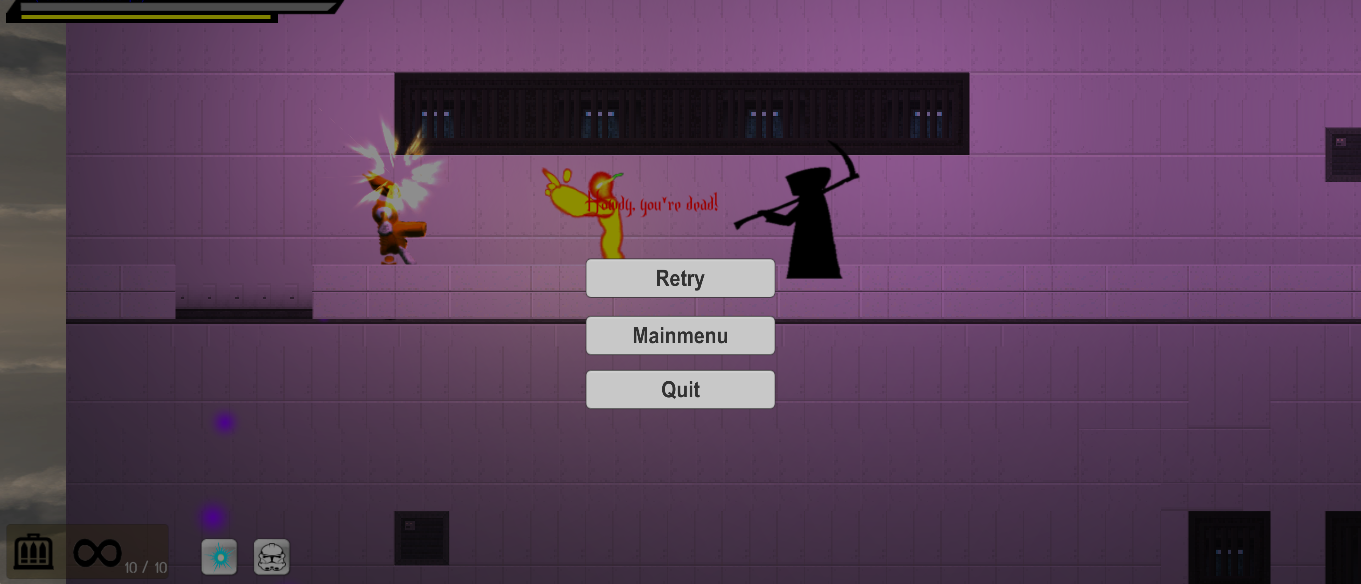
\includegraphics[height=5cm]{images/Todesmenu.png}
	\caption{Todesmenue}
	\label{fig:Todesmenue}
\end{figure}
